% $Id$


Regrid is designed to be called with Field or FieldBundle
arguments in order to utilize information embedded in
these objects.  For example, Regrid requires knowledge
of underlying grid information (both PhysGrid and DistGrid)
and of the relative location (staggering) of Fields on
the Grid.  In addition, Regrid uses any mask information
that may be associated with a Field.  However, ESMF also
provides an Array interface for users who have gathered all
necessary information.

Regrid is separated into RegridStore functions, a Regrid
function, and a RegridRelease function. The Store functions
compute interpolation weights and initialize communication
requirements for performing a regridding of a Field
from one Grid to another, returning an object called an
{\tt ESMF\_RouteHandle}.  The Regrid function uses
the created RouteHandle object to perform the actual regridding
of Fields or FieldBundles.  The Release function deletes the
RouteHandle object and frees all memory associated with a Regrid.
The reason for the separation is that in many cases, the
initial creation is expensive and re-used often throughout
an application.  The Regrid and RegridRelease functions are
also common to all the Regrid methods.

Because many methods are supported for regridding,
the main Store function branches to a specific
creation function based on the regrid method requested
(e.g. bilinear, conservative, spectral).  Each of
these regrid methods are in a separate module to
prevent the main Regrid module from becoming too
large.  The user is unaware of this hierarchy as the
top-level module provides a unified API.

In general, Regrid interfaces are relatively simple and require little
information directly from users.  Besides prescribing the actual Regrid method,
they offer users few options, as shown in the example in
Section~\ref{sec:RegridExamples}.  However, the simplicity of the interfaces
belies the complicated nature of the underlying code.  ESMF endeavors to hide as
much of this complication from its users as possible.  However, Regrid does have
current limitations that require user awareness to successfully use its
routines.  These issues are discussed below.

\subsubsection{Regrid and Grid Overlap}

Regrid assumes both the source and destination Grids share the same coordinate
system and units.  Although 3D regridding is not yet available, this rule is
also expected to be valid for vertical grids as well.  At this point, the ESMF
definition of a common coordinate system includes the extents used to define
a domain.  For example, Regrid routines do not understand that latitudes from
-180 to +180 degrees and latitudes from 0 to 360 degrees are describing the
same domain with a different range.  Currently, users are responsible for any
necessary conversion or translation.  

There are five possible physical overlap situations between the source and
destination Grids, illustrated in Figure~\ref{fig:RegridGridOverlap}.

\begin{center}
\begin{figure}
\scalebox{0.9}{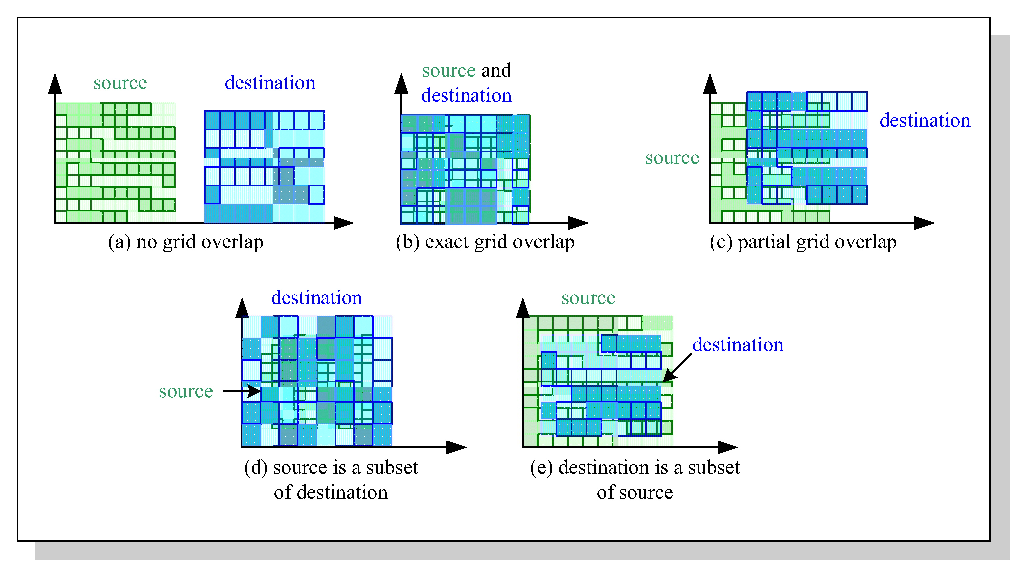
\includegraphics{RegridGridOverlap}}
\caption{Possible Relationships between Grids in Physical (Coordinate) Space. }
\label{fig:RegridGridOverlap}
\end{figure}
\end{center}

Regrid can provide complete interpolation weights for the destination Field
only for those situations where there is source data covering the entire physical
domain of the destination Grid (cases (b) and (e) above).  In all the other
cases, there are parts of the destination Grid for which there is no source. 
When source data is not available, Regrid routines will not extrapolate data
values and the destination Field may contain data points that have not been
calculated or filled.  Currently, regrid routines initialize the destination
Field to a value of zero prior to regridding, so unfilled destination data points
will have that value.  In the future, regrid routines will have an optional
argument allowing users to specify a fill value besides zero.  


\subsubsection{Regrid and Data Location}

There is no restriction in Regrid that the source and destination Fields
define their data in the same relative location (RelLoc).  However, regridding
between Fields with different RelLocs can have unintended consequences if the
related Grids cover exactly the same physical domain.  The RelLocs represent
different subGrids, which can shift the represented physical domain by plus or
minus one-half of a cell width.  This is illustrated below in
Figure~\ref{fig:RegridRelLocEffect}, which shows the physical areas described by
two sample RelLocs and the effect on the overlap of the global Grids.  In this
situation, there may be some unfilled or less accurate Field data at some of the
Grid boundaries.

\begin{center}
\begin{figure}
\scalebox{0.9}{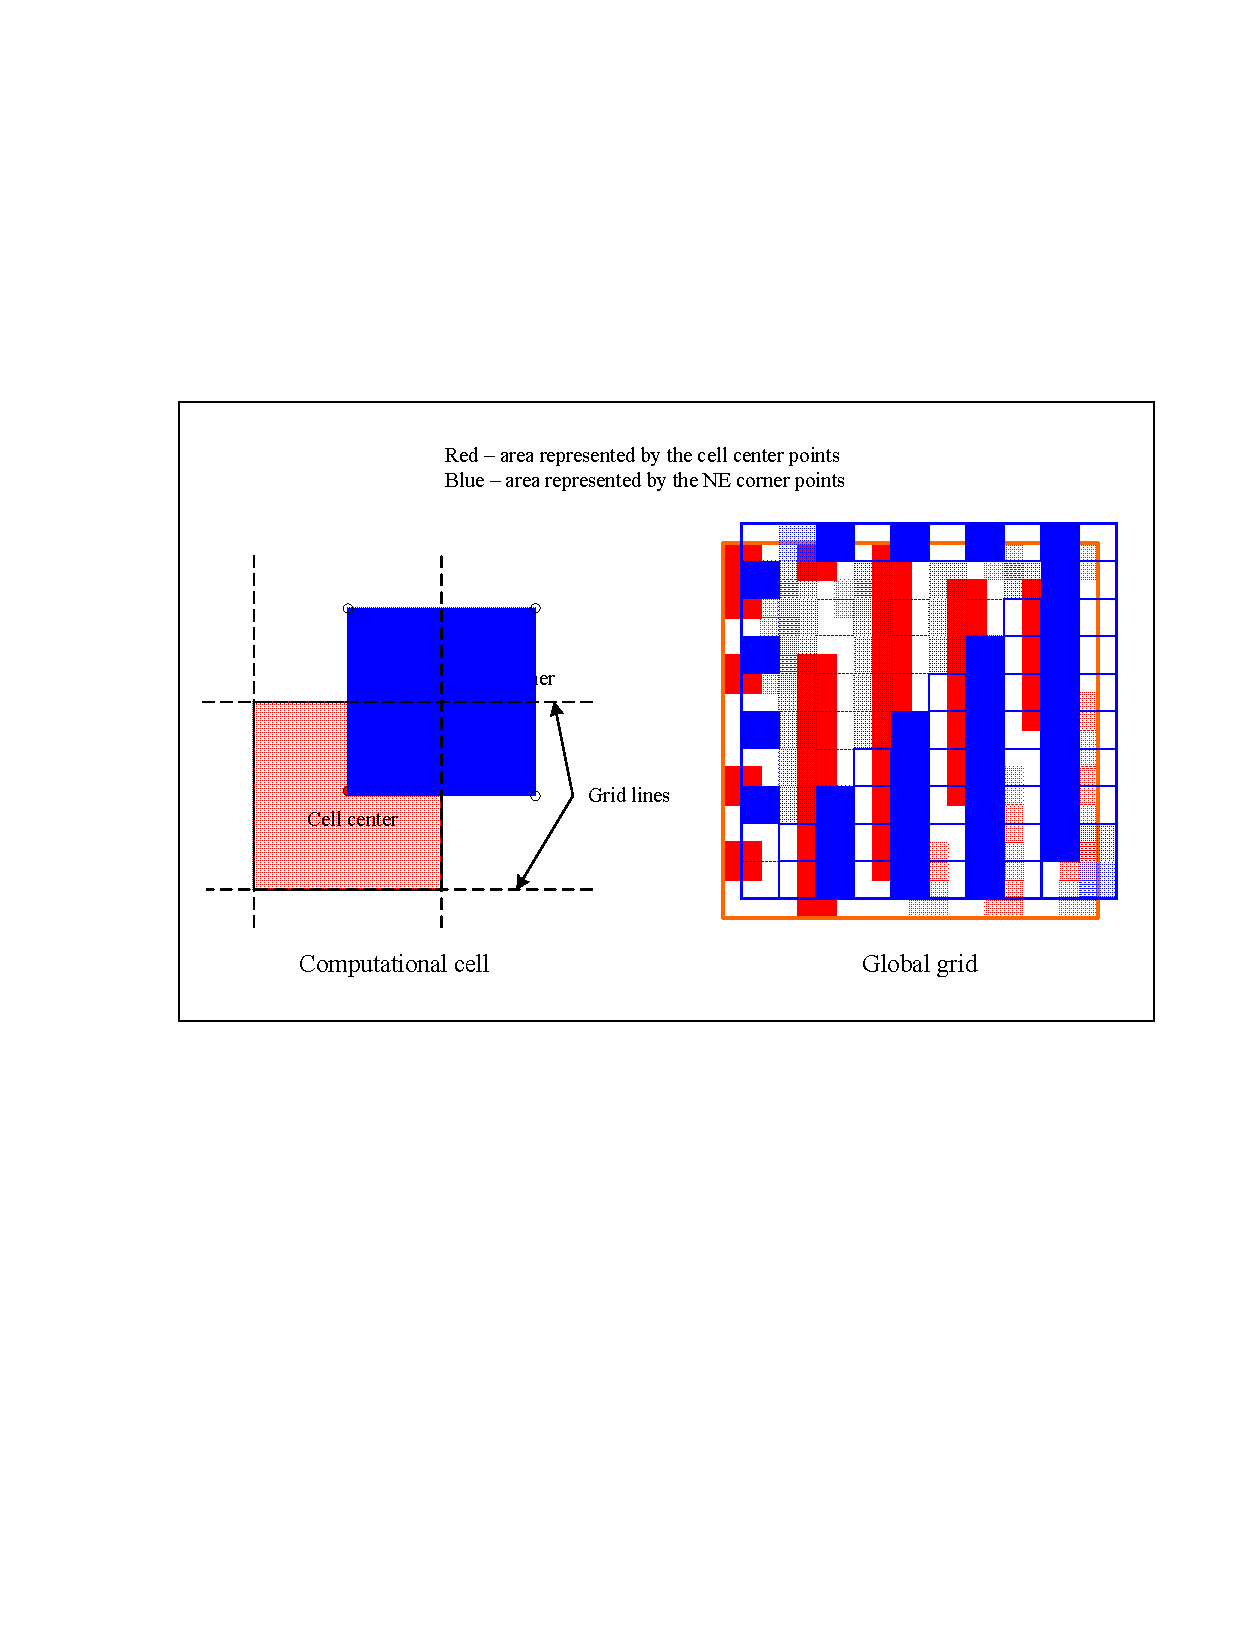
\includegraphics{RegridRelLocEffect}}
\caption{Illustration of Grid areas represented by differing RelLocs. }
\label{fig:RegridRelLocEffect}
\end{figure}
\end{center}

\subsubsection{Regrid and Grid Refinement}

Different refinement or cell sizes (also called resolution) between the source
and destination Grids may have a similar effect on regridding as does different
data locations. This can be true even if the source and destination Fields have
the same RelLoc, as illustrated in Figure~\ref{fig:RegridRefinementEffect}.  In
this diagram, the areas of the two grids represented by the corresponding Fields do not overlap
exactly despite sharing identical physical extents and relative data locations.
Again, this situation may cause some inaccuracy in the regridded Field data at
the Grid boundaries.

\begin{center}
\begin{figure}
\scalebox{0.9}{
\includegraphics{RegridRefinementEffect}}
\caption{Illustration of areas represented by the same RelLoc on Grids with
          different refinement. }
\label{fig:RegridRefinementEffect}
\end{figure}
\end{center}


\subsubsection{Regrid and Periodicity}

Some of the Regrid issues raised in the previous sections concerning the effect
of data locations and Grid refinement are negated by the integration of
periodic boundary conditions into Regrid routines.  As illustrated in
Figure~\ref{fig:RegridPeriodicity}, areas represented by Field data that
would otherwise extend beyond the nominal Grid boundaries are mapped or "wrapped"
back onto the Grid at the corresponding periodic boundary.  This effectively 
ensures complete overlap for Grids that share identical physical extents.

\begin{center}
\begin{figure}
\scalebox{0.9}{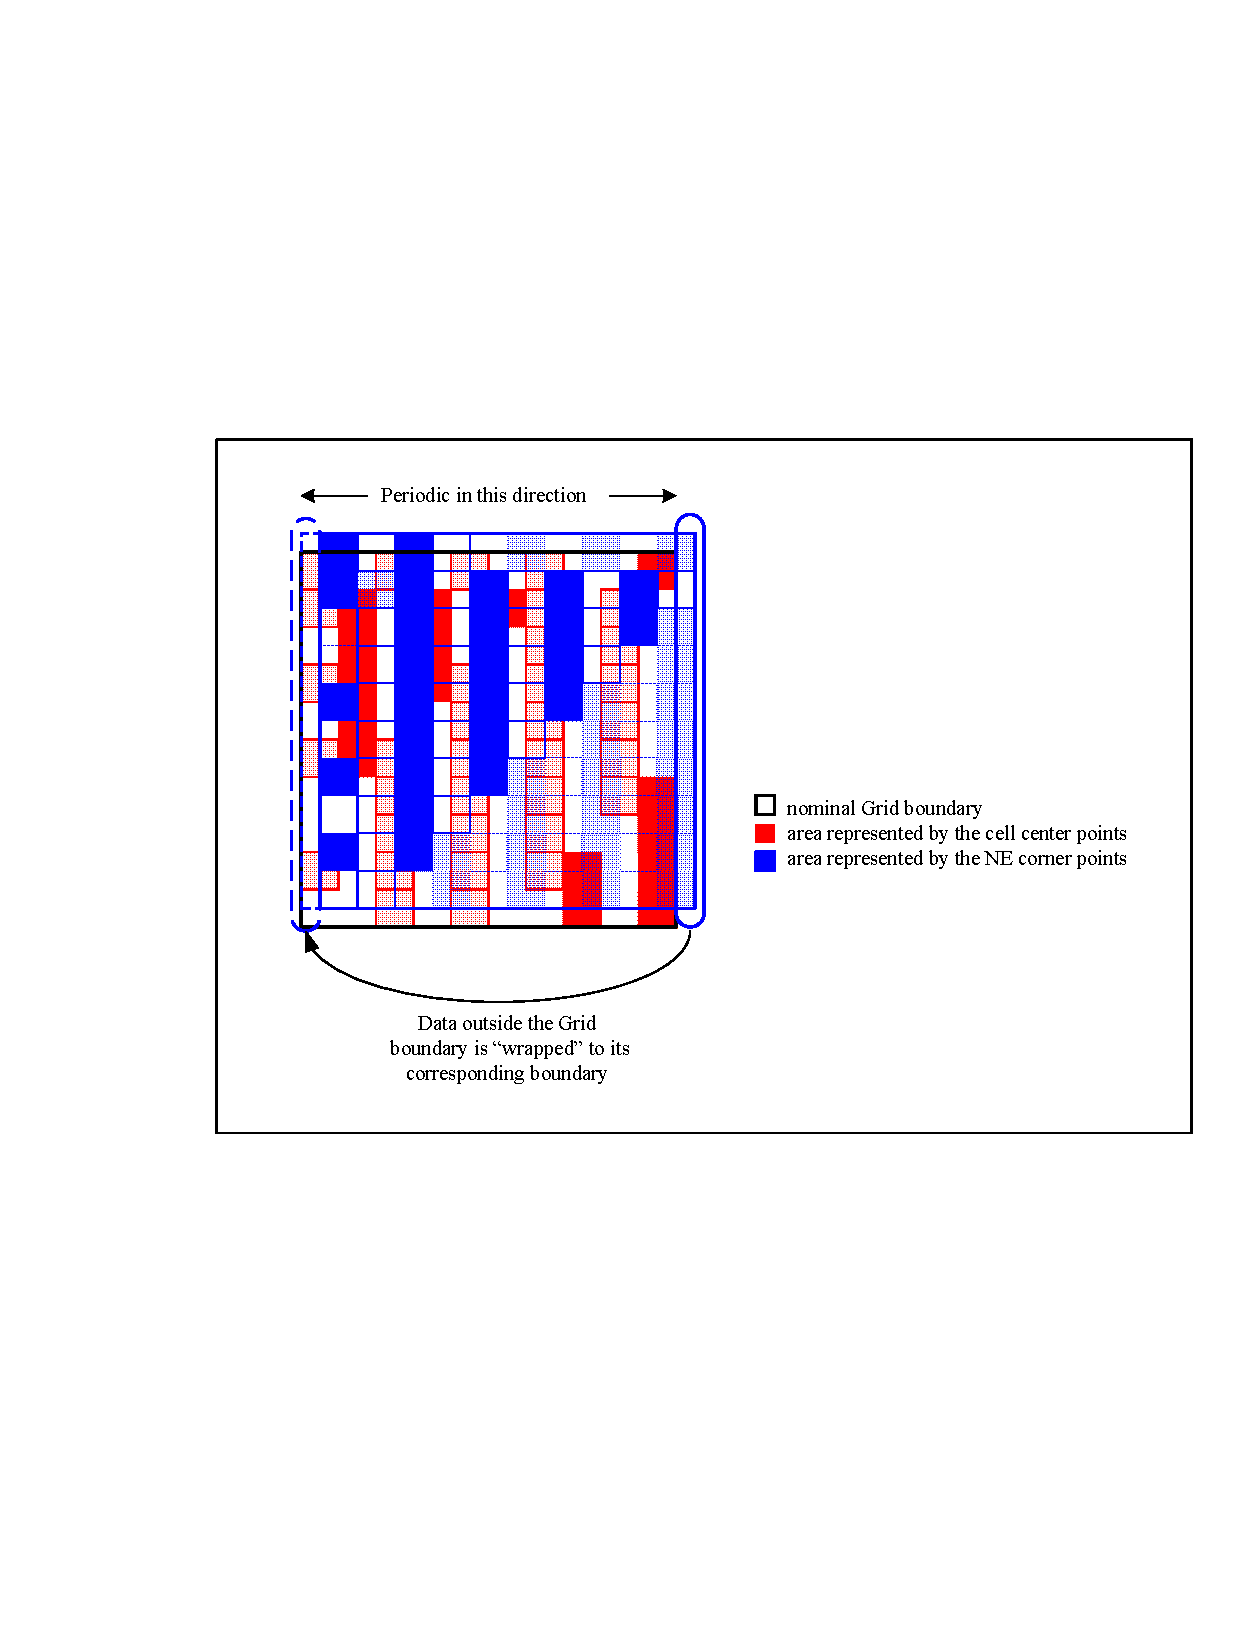
\includegraphics{RegridPeriodicity}}
\caption{Illustration of Regrid Overlap issues solved by the implementation
          of periodic boundary conditions. }
\label{fig:RegridPeriodicity}
\end{figure}
\end{center}

Unfortunately, the Regrid routines in ESMF do not currently include periodic
boundary effects, so users must be aware of possible problems.


\subsubsection{Regrid Examples: Precomputing and Executing a Regrid}
\label{sec:RegridExamples}

The following code fragments show an example of the steps involved in
computing and applying a Regrid.


